\documentclass[10pt, compress]{beamer}

\usepackage{siunitx}
\usepackage{tikz}
\usepackage{pgfplots}
\pgfplotsset{compat=1.13}
\usepackage{booktabs}
\usepackage[scale=2]{ccicons}
\usepackage{minted}

\usetikzlibrary{positioning}
\usemintedstyle{trac}
\usepgfplotslibrary{external} 
\tikzexternalize

%\usefonttheme{professional}
\usetheme{Berlin}
\usecolortheme{dolphin}
\setbeamertemplate{footline}[frame number]
\usepackage{remreset}% tiny package containing just the \@removefromreset command
\makeatletter
\@removefromreset{subsection}{section}
\makeatother
\setcounter{subsection}{1}

\title{Lagging Pendulum}
\subtitle{NZYPT 2016 Problem 1}
\date{\today}
\author{Ernest Wong}
\institute{Macleans College}

\begin{document}

\maketitle




\begin{frame}{The Report at a Glance}
    \begin{center}
    \tableofcontents
    \end{center}
\end{frame}




\section{Preliminary Analysis}



% put problem first
\begin{frame}{The Problem}
    \begin{quote}
        A pendulum consists of a strong thread and a bob. When the pivot of the pendulum starts moving along a horizontal circumference, the bob starts tracing a circle which can have a smaller radius, under certain conditions. Investigate the motion and stable trajectories of the bob.
    \end{quote}
    \pause
    \begin{block}{Keywords}
        \emph{thread, smaller radius, stable trajectories}
    \end{block}
\end{frame}

\begin{frame}{Objective}
    \begin{enumerate}
        \item \textbf{Why} it is possible to have a smaller radius. \alert{(Stability)}
        \item \textbf{How} does the bob end up having a smaller radius. \alert{(Motion and Transitions)}
        \item \textbf{When} does the pendulum enter such state. \alert{(Conditions)}, and what radii that bob can reach.
    \end{enumerate}
\end{frame}

\section{Prelimnary Setup}

\begin{frame}{Preliminary Setup}
    % Photos
    \begin{center}
    \begin{tikzpicture}
        \node[anchor=south west,inner sep=0] (setupimg) at (0,0) {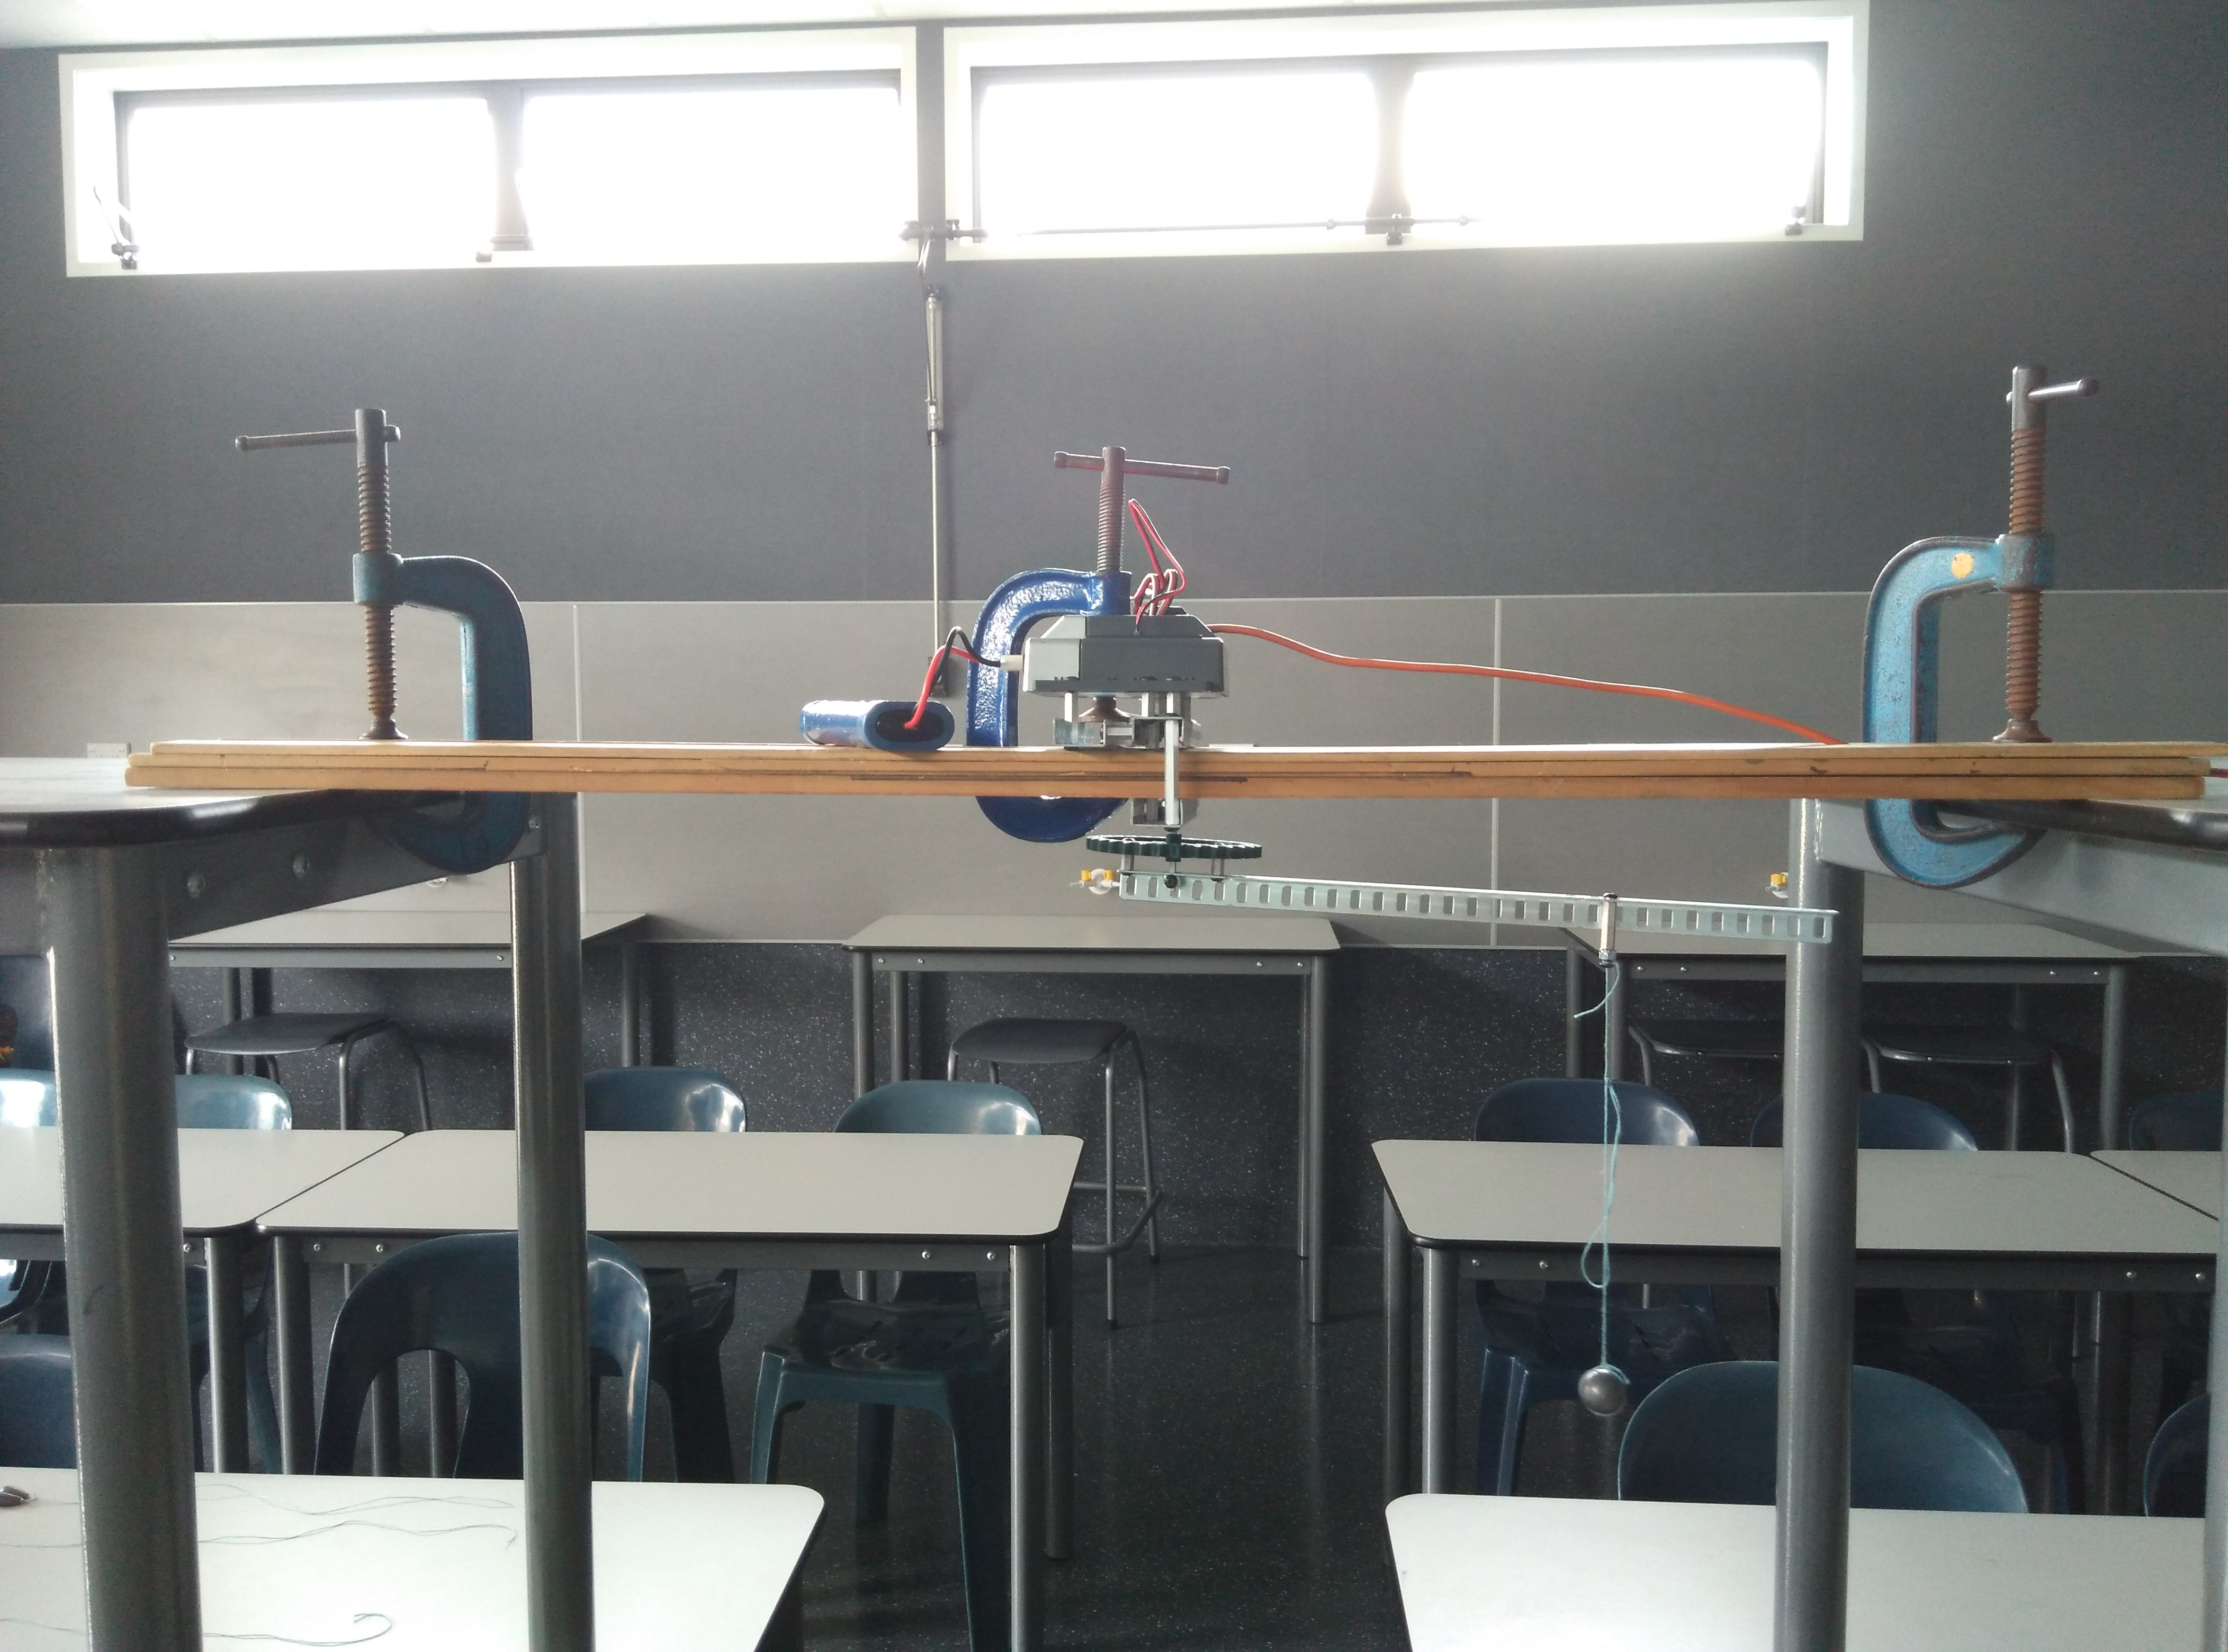
\includegraphics[width=0.9\textwidth]{images/setup.jpg}};
        \begin{scope}[x={(setupimg.south east)},y={(setupimg.north west)}]
            \fill[white,opacity=0.6] (0,0) rectangle (0.4,1);
        \onslide<+->{
            \fill[white,opacity=0.9] (0,0.6) rectangle (0.4,0.7);
            \node at (0.2,0.65) {Self regulated motor};
        }
        \onslide<+->{
            \fill[white,opacity=0.9] (0,0.35) rectangle (0.4,0.45);
            \node at (0.2,0.4) {Pivot arm};
        }
        \onslide<+->{
            \fill[white,opacity=0.9] (0,0.1) rectangle (0.4, 0.2);
            \node at (0.2,0.15) {Threaded bob};
        }
        \end{scope}
    \end{tikzpicture}
    \end{center}
\end{frame}

\begin{frame}{Motor Regulation}
    \begin{center}
    \begin{tikzpicture}
        \node[anchor=south west,inner sep=0] (motorimg) at (0,0) {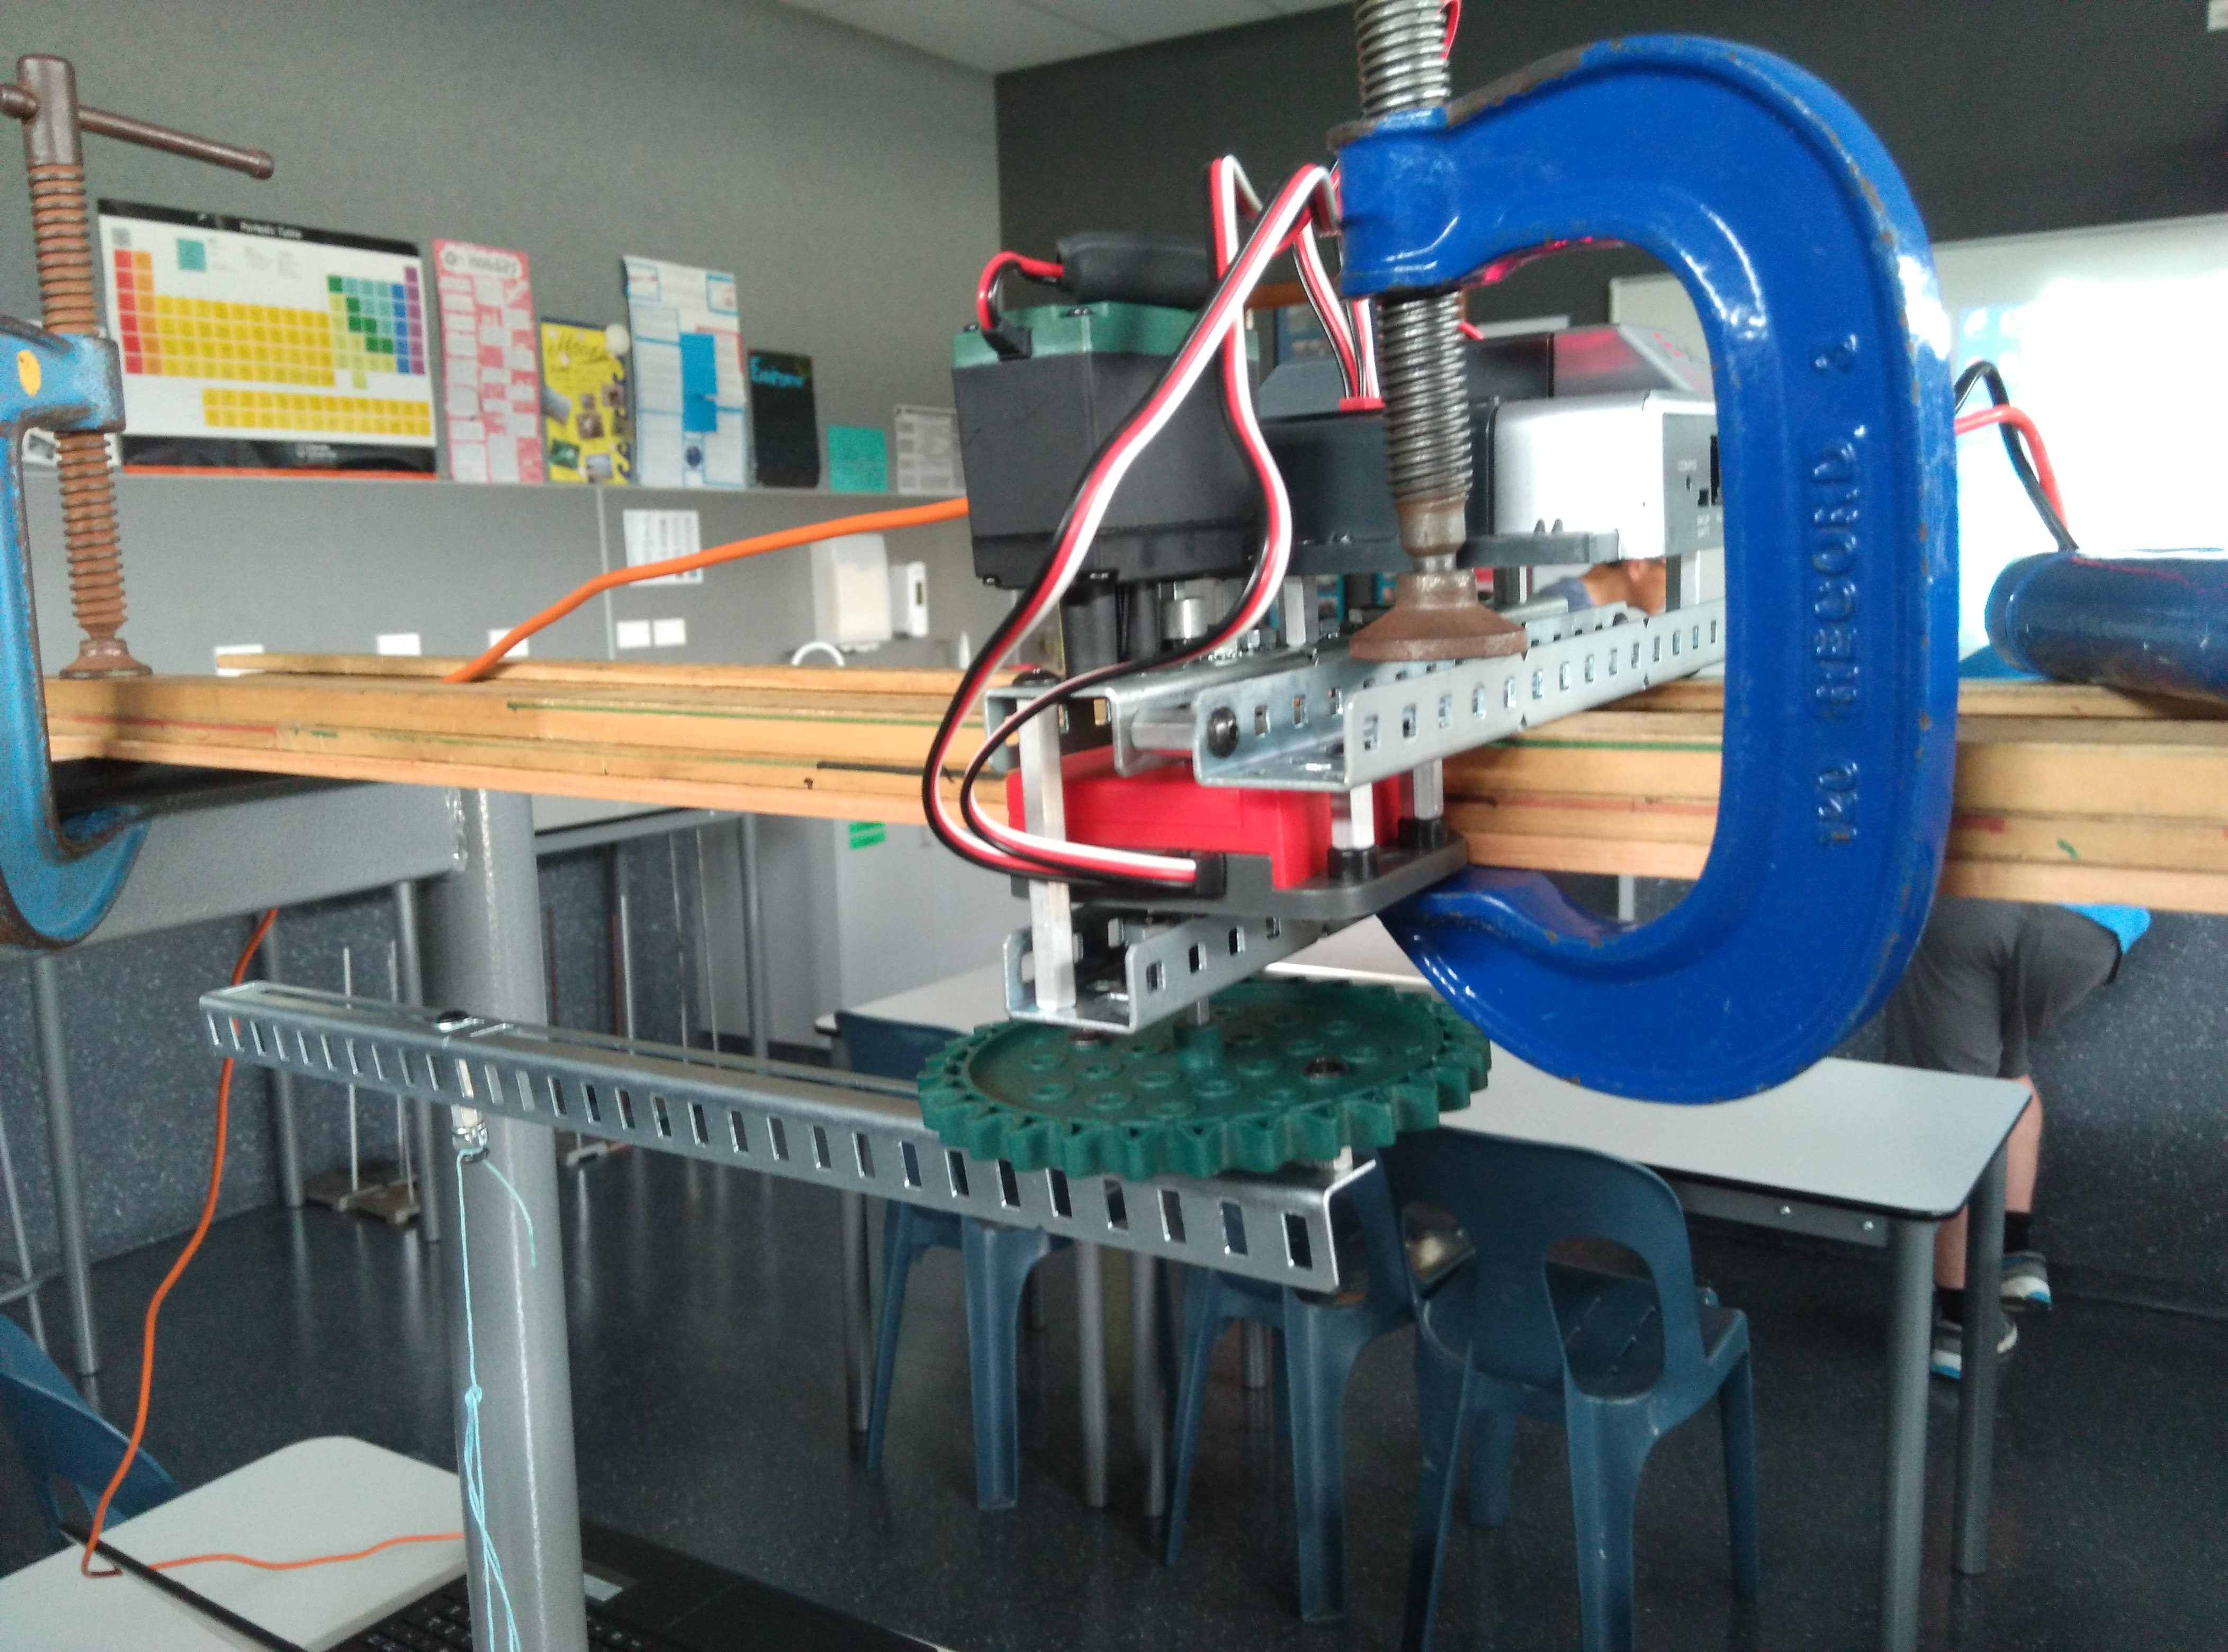
\includegraphics[width=0.9\textwidth]{images/pivoter.jpg}};
        \begin{scope}[x={(motorimg.south east)},y={(motorimg.north west)}]
            \fill[white,opacity=0.6] (0,0) rectangle (0.4,1);
        \onslide<+->{
            \fill[white,opacity=0.9] (0,0.8) rectangle (0.4,0.9);
            \node at (0.2,0.85) {Microcontroller};
        }
        \onslide<+->{
            \fill[white,opacity=0.9] (0,0.65) rectangle (0.4,0.75);
            \node at (0.2,0.7) {Motor};
        }
        \onslide<+->{
            \fill[white,opacity=0.9] (0,0.5) rectangle (0.4, 0.6);
            \node at (0.2,0.55) {Rotatory encoder};
        }
        \onslide<+->{
            \fill[white,opacity=0.9] (0,0.2) rectangle (0.4,0.3);
            \node at (0.2,0.25) {\alert{Negative feedback}};
        }
        \end{scope}
    \end{tikzpicture}
    \end{center}
\end{frame}

\begin{frame}{Data Collection}
    % talk about use of camera, pixel tracking, and transformations with callibration
    \begin{itemize}
        \item Ultra HD 32 FPS Camera (mobile phone) on flat ground
        \item Callibration ruler at known height provides map from pixel to real world rays.
        \item Bisection method to find intersection of ray and sphere
    \end{itemize}
\end{frame}

\section{Steady State Model}

\begin{frame}{Thought Experiment}
    \begin{block}{Assumptions}
    \begin{itemize}
        \item Idealised pendulum: point mass, inextensible massless string, no friction, no drag.
        \item Motion: perfect, horizontal, uniform circular motion, common centre axis.
    \end{itemize}
    \end{block}
    \begin{block}{Results}
    \begin{itemize}
        \item Cannot be same phase: tension outwards.
        \item Very unlikely for different angular velocity.
        \item Other phase differences not steady.
        \item Only 180 deg phase difference.
    \end{itemize}
    \end{block}
\end{frame}

\begin{frame}{Qualitative Model}
    \begin{block}{Equating centripetal force with tension component}
        \begin{equation*}
            \omega^2 = \frac{g}{r_b} \frac{r_b+r_p}{\sqrt{l^2 - (r_b + r_p)^2}}
        \end{equation*}
        {\footnotesize $\omega=\text{Angular velocity of pivot and bob}$, $l = \text{string length}$,and $r_p,r_b=\text{Pivot}$ and bob radius from central axis respectively.}
    \end{block}
    \begin{block}{Numbers from model}
        For $l=\SI{1}{\metre}$, $r_p=\SI{0.12}{\metre}$:
        
        NOTE: Wrong values! use g=9.81
        \begin{center}
        \begin{tabular}{|c|c|c|c|c|}
            \hline
            $r_b / \si{\metre}$ & 0.05 & 0.10 & 0.15 & 0.30 \\
            \hline
            $\omega / \si{\radian\per\second}$ & 8.28 & 6.82 & 6.37 & 7.00 \\
            \hline
        \end{tabular}
        \end{center}
    \end{block}
\end{frame}

\begin{frame}{Preliminary Observations}
    Testing with mass $m=\SI{61}{\gram}$, $l=\SI{51}{\centi\metre}$, $r_p=\SI{12}{\centi\metre}$:
    
    \begin{center}
    \begin{tabular}{c c}
        \hline
        $\omega / \si{\radian\per\second}$ & Observation \\
        \hline
        5.24 & Radius increased, exceeded setup's boundaries\\
        6.28 & Radius increased, exceeded setup's boundaries\\
        7.33 & Radius increased, exceeded setup's boundaries\\
        8.38 & Radius increased, exceeded setup's boundaries\\
        \hline
    \end{tabular}
    \end{center}
    
    Need further investigation, so we turn to numerical model.
\end{frame}

\section{Numerical Analysis}

\begin{frame}{Mathematical Model}
    Lagrangian:
    \begin{equation*}
        L = \tfrac{1}{2}m\left(\dot{x}^2 + \dot{y}^2 + \dot{z}^2\right) - mgz_p + mgl\cos\theta.
    \end{equation*}
    Using Euler-Lagrange equations, we get the equations of motion:
    \begin{block}{Generalised}
    \begin{align*}
        \ddot{\theta} &= \dot{\phi}^2 \sin\theta\cos\theta
            - \frac{
                \ddot{x_p}\cos\theta\cos\phi + \ddot{y}_p\cos\theta\sin\phi +
                (g + \ddot{z}_p)\sin\theta}{l}\\
        \ddot{\phi} &= \frac{\sin(\phi_p-\phi)}{l\sin\theta} - 2 \frac{\dot{\phi}\dot{\theta}}{\tan\theta}
    \end{align*}
    \end{block}
\end{frame}

\begin{frame}{Mathematical Model}
    \begin{block}{EOM for lagging pendulum}
    \begin{align*}
        \ddot{\theta} &= \dot{\phi}^2 \sin\theta\cos\theta + \frac{r_p}{l} \omega^2 \cos\theta\cos(\phi-\phi_p) - \frac{g}{l}\sin\theta\\
        \ddot{\phi} &= \frac{\sin(\phi_p-\phi)}{l\sin\theta} - 2 \frac{\dot{\phi}\dot{\theta}}{\tan\theta}
    \end{align*}
    \end{block}
\end{frame}

\begin{frame}{Numerical Model}
    \begin{block}{EOM for lagging pendulum \alert{+ energy dissipation}}
    \begin{align*}
        \ddot{\theta} &= \dot{\phi}^2 \sin\theta\cos\theta + \frac{r_p}{l} \omega^2 \cos\theta\cos(\phi-\phi_p) - \frac{g}{l}\sin\theta \alert{- b_\theta \dot{\theta}}\\
        \ddot{\phi} &= \frac{\sin(\phi_p-\phi)}{l\sin\theta} - 2 \frac{\dot{\phi}\dot{\theta}}{\tan\theta} \alert{- b_\phi \dot{\phi}}
    \end{align*}
    \end{block}
    Numerically solved using Runge Kutta 4th Order Algorithm.
\end{frame}

\begin{frame}{Observations in simulation}
    Polar angle oscillates, and converges to steady state.
\end{frame}

\begin{frame}{Hypothesis: Phase difference \& Polar Angle}
    Todo: add beautiful diagrams.
    Phase difference pulls bob, accelerates and lead to higher polar angle.
\end{frame}

\begin{frame}{Simulation: Phase difference \& Polar Angle}
    Todo: add beeautiful plot.
    %\includegraphics[width=\textwidth]{phasediff-angle1.png}
    \begin{tikzpicture}
    \begin{axis}
        \addplot table[x=anglediff,y=dangle1,col sep=comma]{data/phasediff-dangle1.csv};
    \end{axis}
    \end{tikzpicture}
\end{frame}

\section{Stability}

\begin{frame}{State Approximation}
    State of the pendulum can be described by $(\theta, \dot\theta, \phi, \dot\phi, \phi_p)$.
    
    But near-steady-state: roughly circular, so $\dot\phi$ can be approximated, i.e. using:
    
    \begin{equation*}
        \dot\phi \approx \sqrt{\frac{g\tan\theta}{l\sin\theta + r_p}},
    \end{equation*}
    
    Hence, overall state can be simplified to $(\theta, \dot\theta, \phi - \phi_p)$.
\end{frame}

\begin{frame}{Behaviour using near-steady-state approximation:}
    \begin{block}{When $\phi > \phi_p$}
        $\theta$ \alert<2>{increases}. \\
        If $\dot\phi$ increases, then \textbf{positive feedback}. \\
        If $\dot\phi$ \alert<2>{decreases}, the \textbf{negative feedback}.
    \end{block}
    \begin{block}{When $\phi < \phi_p$}
        $\theta$ \alert<2>{decreases}. \\
        If $\dot\phi$ \alert<2>{increases}, then \textbf{negative feedback}. \\
        If $\dot\phi$ decreases, the \textbf{positive feedback}.
    \end{block}
    Stable if \alert<2>{negative feedback}.
\end{frame}

\section{Stability}




\begin{frame}{Angular Velocity --- Regular Conical Pendulum}
    \begin{block}{$\text{Equating centripetal}=\text{resolved}$}
        \begin{equation*}
            \omega^2 = \frac{g}{\sqrt{l^2 - r^2}}
        \end{equation*}
    \end{block}
    \only<1>{
        \begin{center}
        \begin{tikzpicture}[scale=1.5]
            \coordinate (O) at (0,0);
            \draw[fill=fg] (O) circle (0.2mm);
            \draw (O) -- +(250:2cm) node[midway,above left] {length $l$} coordinate (B);
            \node[above] at (O) {pivot};
            \node[left=4mm of B] {bob};
            \draw[fill=bg] (B) circle (2mm);
            \draw[->] (B) arc (210:310:8mm and 2mm) node[below right] {angular velocity $\omega$} coordinate (C);
            \draw[dashed] (C) arc (310:500:8mm and 2mm);
            \coordinate[below=5mm of B] (BB);
            \draw[<-|] (BB) -- (BB-|O) node[midway,below] {radius $r$};
        \end{tikzpicture}
        \end{center}
    }
    \onslide<2->{
        \begin{columns}[c]
        \uncover<2->{
            \begin{column}{0.45\textwidth}
                \begin{block}{Changing Radius (const. $l$)}
                \begin{center}
                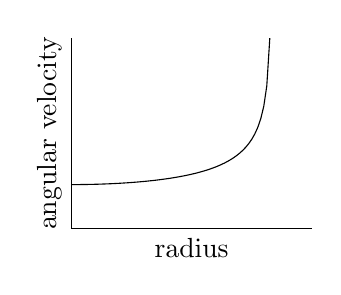
\begin{tikzpicture}
                    \begin{axis}[
                        axis lines=left,
                        height=4cm,
                        ticks=none,
                        axis line style={-},
                        xlabel=radius,
                        ylabel=angular velocity,
                        xmin=0,
                        xmax=1.2,
                        ymin=0.5
                    ]
                        \addplot[
                            domain=0:3,
                            samples=201
                        ]
                            {sqrt(1/sqrt(1-x^2))};
                    \end{axis}
                \end{tikzpicture}
                \end{center}
                \end{block}
            \end{column}
        }
        \uncover<3>{
            \begin{column}{0.45\textwidth}
                \begin{block}{Changing length (const. $r$)}
                \begin{center}
                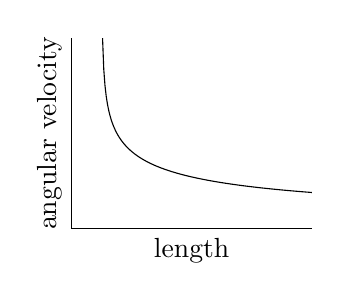
\begin{tikzpicture}
                    \begin{axis}[
                        axis lines=left,
                        height=4cm,
                        ticks=none,
                        axis line style={-},
                        xlabel=length,
                        ylabel=angular velocity,
                        xmin=0,
                        xmax=8,
                        ymin=0
                    ]
                        \addplot[
                            domain=0:8,
                            samples=201
                        ]
                            {sqrt(1/sqrt(x^2-1))};
                    \end{axis}
                \end{tikzpicture}
                \end{center}
                \end{block}
            \end{column}
        }
        \end{columns}
    }
\end{frame}

\begin{frame}{Angular Velocity --- Our Case Qualitatively}
    As bob radius $r_b$ increases, effective length $l_b$ also increases.
    
    \begin{center}
    \begin{tikzpicture}
        \coordinate (O) at (0,0);
        \draw (O) ellipse (12mm and 3mm);
        \coordinate (P) at (12mm, 0);
        \draw[fill=fg] (P) circle (0.5mm) node[right] {pivot};
        \draw[opacity=0.1] (P) -- +(240:40mm) coordinate (A);
        \draw[opacity=0.5] (P) -- +(230:40mm) coordinate (B);
        \draw[opacity=1.0] (P) -- +(220:40mm) coordinate (C);
        \draw[dashed] (A-|O) -- (O);
        \draw[opacity=0.1] (A) -- (A-|O);
        \draw[opacity=0.5] (B) -- (B-|O);
        \draw[opacity=1.0, thick] (C) -- (C-|O) node[midway,above] {$r_b$};
        \coordinate (CP) at (intersection cs:
            first line={(C)--(P)},
            second line={(O)--(A-|O)});
        \draw[fill=fg] (CP) circle (0.5mm);
        \draw[ultra thick] (CP) -- (C) node[midway,above left] {$l_b$};
        \draw[fill=bg,draw opacity=0.1] (A) circle (2mm);
        \draw[fill=bg,draw opacity=0.5] (B) circle (2mm);
        \draw[fill=bg,draw opacity=1.0] (C) circle (2mm);
    \end{tikzpicture}
    \end{center}
    
    Therefore, $(r_b \to \omega)$ isn't monotonic.
\end{frame}

\begin{frame}{Angular Velocity --- Our Case Quantitatively}
    \begin{columns}[t]
        \begin{column}{0.5\textwidth}
        \begin{block}{Assumptions}
            \begin{itemize}
                \item Perfect uniform, horizontal, circular motion.
                \item No air drag/friction.
                \item Ideal string.
                \item Point mass.
            \end{itemize}
        \end{block}
        \end{column}
        \begin{column}{0.5\textwidth}
        \begin{block}{Result}
            \begin{equation*}
                \omega^2 = \frac{g}{r_b} \frac{r_b+r_p}{\sqrt{l^2 - (r_b + r_p)^2}}
            \end{equation*}
        \end{block}
        \end{column}
    \end{columns}
\end{frame}

\begin{frame}{Angular Velocity --- Plot}
    \begin{center}
    \begin{tikzpicture}
        \begin{axis}[
            axis lines=left,
            height=75mm,
            xlabel=$r_b$,
            ylabel=$\omega$,
            xmin=-6,
            xmax=4,
            ymin=0,
            ymax=6,
            xtick={0},
            ytick={0}
        ]
            \only<1-2> {
                \addplot[
                    domain=-6:-1,
                    samples=401
                ]
                    {sqrt(10/x*(x+1)/sqrt(16-(x+1)^2))};
            }
            \only<1,3> {
                \addplot[
                    domain=0:4,
                    samples=401
                ]
                    {sqrt(10/x*(x+1)/sqrt(16-(x+1)^2))};
            }
            \coordinate (MINW) at (axis cs:1.52,2.31);
            \only<2> {
                \addplot[
                    domain=0:4,
                    samples=401,
                    opacity=0.1
                ]
                    {sqrt(10/x*(x+1)/sqrt(16-(x+1)^2))};
            }
            \only<3> {
                \addplot[
                    domain=-6:-1,
                    samples=401,
                    opacity=0.1
                ]
                    {sqrt(10/x*(x+1)/sqrt(16-(x+1)^2))};
                \draw[fill=fg] (MINW) circle (0.4mm);
                \node[below=0.8mm of MINW] {$r_b=\sqrt[3]{l^{2}r_p^{3}}-r_p$};
            }
            \node[rectangle,draw] at (axis cs:-2.5,5) {$\omega^2 = \frac{g}{r_b} \frac{r_b+r_p}{\sqrt{l^2 - (r_b + r_p)^2}}$};
            \only<2> {
                %\fill[bg,opacity=0.9] (axis cs:-0.1,0) rectangle (axis cs:4,6);
                \pgfplotsinvokeforeach{1,2,3,4} {
                    \draw[<-,ultra thick] (axis cs:0,##1) -- (axis cs:0.7,##1);
                }
            }
            \only<3> {
                %\fill[bg,opacity=0.9] (axis cs:-0.1,0) rectangle (axis cs:4,6);
                \pgfplotsinvokeforeach{2,3,4} {
                    \draw[->,ultra thick] (axis cs:-1.7,##1) -- (axis cs:-1,##1);
                }
            }
        \end{axis}
    \end{tikzpicture}
    \end{center}
\end{frame}

\begin{frame}{Testing minimum $\omega$}
\begin{enumerate}
    \item For each $r_p$, get max $\omega$ and set up pendulum.
    \item Decrease $\omega$ gradually until bob's circular trajectory collapses, and record $\omega$ to get $\omega_{\text{min}}$.
\end{enumerate}
\end{frame}

% http://www.zn.dmef.put.poznan.pl/content/009/009.pdf
% Found the lagrangian and solved it, and checked with
% R. Mitrev, B. Grigorov.
% DYNAMIC BEHAVIOUR OF A SPHERICAL PENDULUM WITH SPATIALLY MOVING PIVOT 

\section{Transitions}

\section{Conditions}

\end{document}
